%%% 1 Introduction/ %%%
\chapter{Introduction}\label{ch:intro}
%WHAT - what the reader needs to know to understand the presented 
%work, explain the background of research
%Society, Honesty difficult to predict, spy problem.
%only way - to constantly get feedback about the current behavior
%prisoner's dilemma an expermient that suggests, people act honestly if there is 
% long term benefit 
%i.e., if a user might have to interact again with the same person for some
%reason, then they are more likely to behave honestly. 
From using emails to communicate with one another, searching for an online
source to get the news or media files to shopping for everyday things, we rely
heavily on the internet today. One can say that the internet has become an
inseparable part of our society. Statistics~\cite{InternetWorldStat} suggest
that there are approximately 4 billion internet users worldwide and this number
is only increasing with each passing day. Internet live
stats~\cite{InternetLiveStat} is an online service that provides live
statistics on various online activities such as blog posts, social media usage,
internet traffic and emails sent. Given the global reach of the internet and
diversity of users, one can reasonably assume that not all online interactions
happen between known entities. The online identities that everyone uses to
interact with one another provide no way to confirm the real-world identity or
the attitude of the person behind. To determine the trustworthiness of an
entity is a difficult task even in the real world. If Alice needs to interact
with Bob, she has no way of actually measuring the trustworthiness of Bob with
100\% certainty. One way to do that is to get a reference from others in the
society, i.e., by referring to Bob's reputation. If Bob has a good standing
among members of the community due to good records or other objective measures,
there is a high probability that Alice's interaction with Bob will result in a
good outcome. i.e., Alice's perception of Bob will turn out to be true.
However, this doesn't provide any guarantee of Bob's behavior. Bob could be a
malicious actor in a society who was waiting for the right moment to deal
severe damage. There is no way of guaranteeing that the behavior of an entity
will always be an honest one. Honesty can be seen as an attribute at a given
time. Alice may trust Bob today but not tomorrow because of certain actions.
Depending on the action and damage caused, the level of trustworthiness also
gets affected. As such, we can say that anyone is honest until they deal damage
to be known as a malicious actor in the society. That is when they lose their
reputation, and other members are less likely to trust them. \par 
\begin{figure}
	\begin{center}
		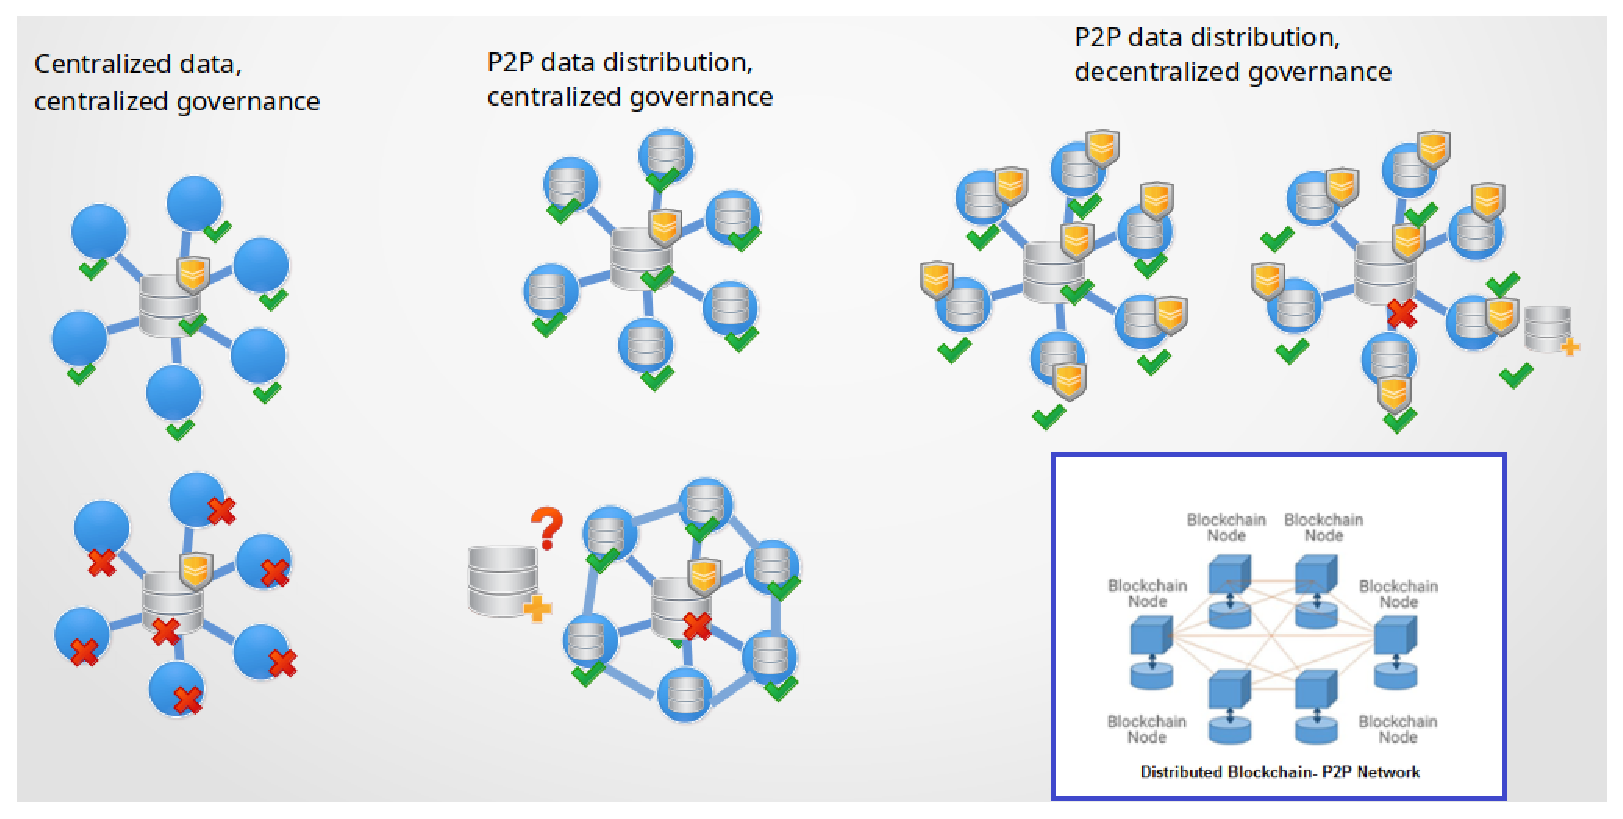
\includegraphics[width=1.0\textwidth]{Images/WhyBlockchain.eps}
		\caption{Centralized Vs. decentralized network}
		\label{fig:WhyBlockchain}
	\end{center}
\end{figure}
This notion of trust and reputation, when used in online interactions, can help
to predict the outcome of online transactions. Any online platform where users
communicate with each other for different purposes (e.g., digital transaction,
news or file sharing) can be termed as online interaction system. Depending on
the nature of the interaction, the outcome can have a significant impact on
interacting entities. For instance, the failure of an interaction that involves
buying a house is not the same as failing to receive a high-quality music file.
To prevent severe damage that might result from a failed transaction, trust
frameworks and reputation model of the interaction system plays a crucial role.
They attempt to avoid harm by giving enough information about the interacting
entities to be able to predict the outcome. A reputation system collects
information about the interacting entities continuously by continually updating
the state based on feedbacks. The risk of failure or probability of success
when transacting with an entity is reliant on the information provided by the
underlying reputation system. This information is usually presented in the form
of trust scores assigned to each online identities. Before engaging in an
online transaction, the entities need to select the online identity of the user
with whom they intend to interact. The interaction can then take place whose
outcome is observed and stored by the reputation system to update the current
trust value further. Examples of reputation systems in use by current online
interaction platform are eBay~\footnote{https://www.ebay.com/}, which is an
e-commerce platform, StackExchange~\footnote{https://stackexchange.com/}, which
is a Q\&A platform, and Reddit~\footnote{https://www.reddit.com/}, which is a
content rating and discussion platform. The trust score of users is based on
their feedback, positive/negative ratings, upvotes/downvotes from the
participants with an equal privilege to interact with the system. The final
score aggregated via these objective measures can either increase or lower the
reputation of the user and limit their interaction ability. \par 

A general trust framework and a good reputation model to specify the rules of
interaction between online identities and the extraction of useful information
from them is, therefore, essential to maintaining the security of an online
interaction system. Equally significant is to protect the integrity of this
information such that they are reliable, untampered (no deliberate alteration
of data) and always available. Most of the online interaction systems make use
of a client-server architecture to serve and govern the data usage. As such,
the system is centralized and prone to both external attacks and internal
modifications. If the server node fails, then the whole network fails since
none of the clients can access the data anymore. An alternative architecture
that is primarily utilized by file sharing systems is a Peer-to-Peer (P2P)
network, and reputation-based trust management system for them exists as
well~\cite{selcuk2004reputation}. In a P2P network, all nodes (peer) can act as
both client and server, i.e., a peer can both request and serve data. Thus, if
one node fails then, clients can still request data from other nodes in the
network. This architecture solves the problem by P2P data distribution.
However, the governance of data is still centralized such that clients still
need to wait for a particular node that has the privilege to add new data. This
leaves the possibility for an online service running on these networks to be
shut down or data to be modified by the central authority. Examples include the
shutdown of P2P services such as KaZaA~\cite{mlcakova2004configuring} and
Napster~\cite{stern2000napster}. Therefore, this system is still vulnerable to
internal modifications as it is reliant on a trusted entity (special node to
add data). Blockchain~\cite{atzori2015blockchain} solves these issues by
providing P2P data distribution along with decentralized data governance. 
The figure~\ref{fig:WhyBlockchain} in section~\ref{ch:intro} shows the difference between the models mentioned above. \par
\begin{figure}
	\begin{center}
		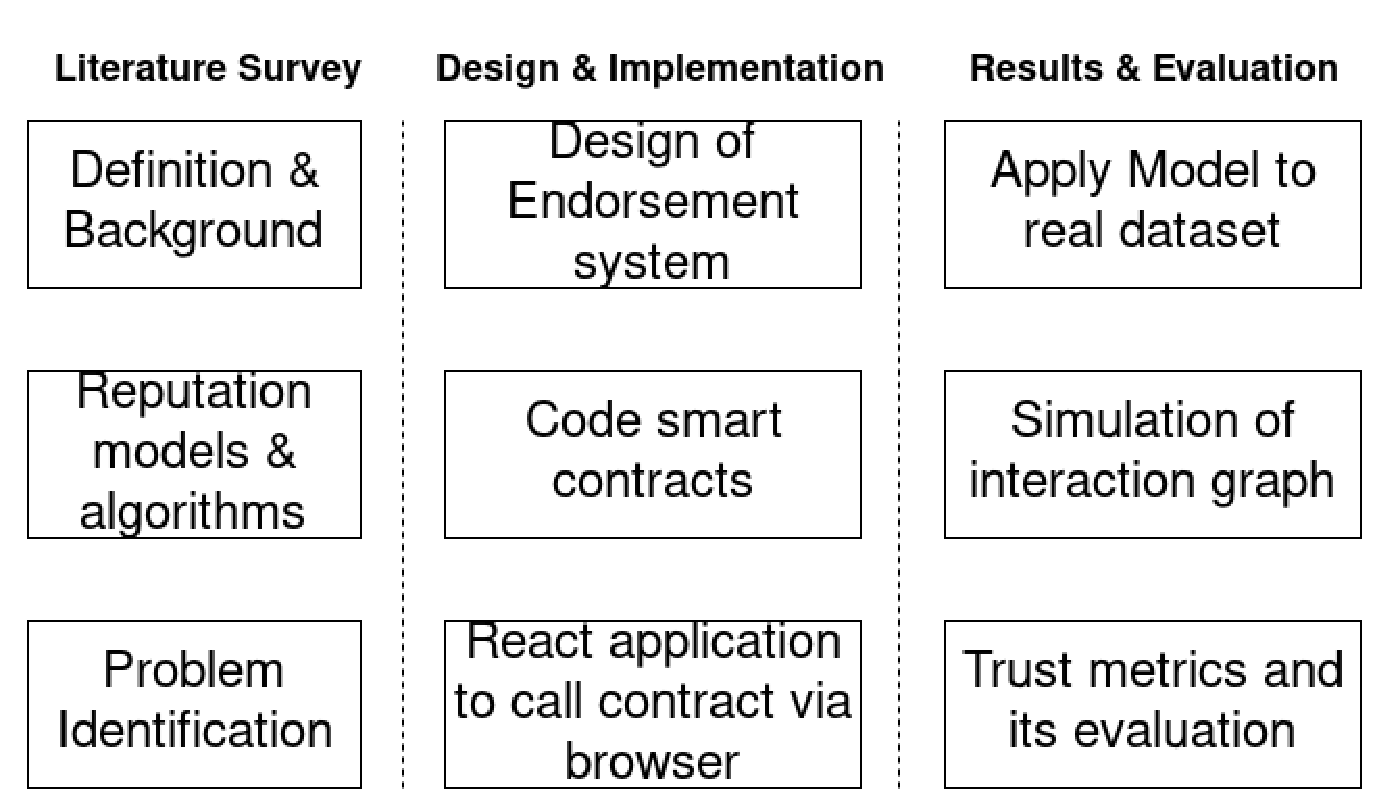
\includegraphics[width=0.9\textwidth]{Images/workflow.eps}
		\caption{Workflow of the project's phases}
		\label{fig:thesisSteps}
	\end{center}
\end{figure}
This master’s thesis project, therefore, proposes the use of blockchain
technology and smart contracts to model a trust framework and implement a
reputation system. The initial step of the project was the identification of
relevant concepts by performing a literature survey on existing reputation
models, properties of graph-based algorithms and its relevance to the project.
The survey motivated the design of a solution, wherein the proposed model,
participating entities can endorse each other. Based on assumptions about
different possibilities of endorsement behavior that may occur, trust metrics
were defined in a way that honest participation would be encouraged. The
definition of honest and malicious participation from the perspective of an
endorsement network is discussed. A method to collect and quantify this
endorsement information to assign a trust score to each entity is presented. To
assess the working of the proposed model, it is applied to an existing real
dataset. Computation of trust scores for each participant based on the defined
trust metrics is presented. The simulated graph and computed trust scores do
support the defined metrics. A discussion of relevant threat models on
reputation systems and how the proposed model addresses them is performed. The
figure~\ref{fig:thesisSteps} in section~\ref{ch:intro} gives the workflow of
this master’s thesis project. \par

The major contribution of this master's thesis project is:
\begin{itemize}
	\item Design of an endorsement model where entities can endorse each
		other's information and a method to aggregate this information such
		that a global value can be assigned to individual entities to infer
		their trustworthiness. 
	\item Deployment of the endorsement system on blockchain network that
		updates and computes the trust scores of entities by executing the
		smart contract code based on user's interaction ensuring reliable and
		verifiable information. 
	\item Evaluation of the endorsement model by applying it to an existing
		data set and discussion of relevant threat model
\end{itemize}

%and therefore can be stated as a soft
%security mechanism. Rasmusson, Lars and Jansson,
%Sverker~\cite{rasmusson1996simulated} first used this term to describe the idea
%of identifying malicious users and preventing harm to other users in the
%context of secure open electronic commerce. Here, it is up to the individuals
%rather than the software to maintain security.

%\begin{wrapfigure}{l}{0.6\textwidth}
%	\begin{center}
%		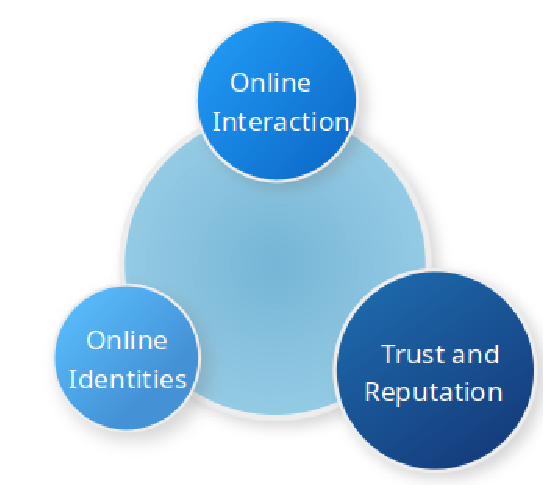
\includegraphics[width=0.5\textwidth]{Images/Introduction.eps}
%		\caption{Online identities and their interaction}}
%		\label{fig:introduction}
%	\end{center}
%\end{wrapfigure}
 
\section{Motivation}
%WHY: why is it interesting to study reputation system/trust 
% why blockchain based solution is relevant/interesting
Consider a simple scenario where Alice wants to buy a pair of headphones for
which she browses a ``buy/sell'' platform. When she finds a relevant product on the
platform published by Bob, unknown entity to Alice, the success or failure of
the transaction is dependent on two factors that may or may not be transparent.
\paragraph{Bob's reputation:}Bob's reputation can be inferred from his history
of transactions, ratings provided by previous buyers that have dealt with him,
reputation system of the platform in use, the integrity of all these relevant
data.  
\paragraph{Platform's reputation:}Reputation of the platform can also be
inferred similarly based on the history of services it has been able to
provide, a general perception in the community, etc.  Here, the platform in use
acts as the trusted third party that Alice must trust to present correctly
computed, untampered data about Bob. The entity claiming to be Bob could be
Eve, who found a way to bypass the platform's security and inflate his
reputation.  Eve could delete the ad and associated account when the payment is
complete, or she could gather Alice's details to misuse it later.  Any
malformed decision on the trustworthiness of an entity could be expensive and
deal severe damage to the user. \par 
Statistics suggest that online shopping is the most adapted online
activity~\cite{experian}. Reports by Experia~\cite{experian} and
Javelin~\cite{javelin} indicate that E-commerce fraud has risen to
30\% in 2017 from 2016 while identity fraud victims have risen by 8\% in 2017
(16.7 million U.S victims). 
%Additionally, reports on fake news
%\footnote{\url{https://journalistsresource.org/studies/society/internet/fake-news-conspiracy-theories-journalism-research}}$^{,}$\footnote{\url{https://www.prnewswire.com/news-releases/84-percent-of-businesses-could-reduce-fraud-risk-if-certain-about-customers-identity-300587192.html}}
%that leads to spread of misinformation from malicious users or portals, attack
%on an existing system continues.
A recent report of data breach on Finnish Enterprise Agency for
Helsinki~\cite{finland}~\footnote{https://liiketoimintasuunnitelma.com/}
exposed 130,000 users login details.
%while Facebook has admitted to the compromise of
%2.2 billion of its user's data
%\footnote{\url{https://thenextweb.com/facebook/2018/04/05/zuckerberg-facebooks-2-billion-users-assume-data-compromised/}}.
%\footnote{\url{https://thehackernews.com/2018/04/facebook-data-privacy.html}}.
While there are several security reasons that have led to attack at such scale.
One major reason is the client-server architecture where everything is stored
on a centralized server and data flows in and out from the same source. On the
other hand, distributing information over a decentralized network would require
a simultaneous attack to achieve the same effect, thereby increasing the
difficulty level of attack. Similarly, Reputation models can help in measuring
the reliability of interacting entities so that users can make an informed
decision before participating in any transactions. Thus, a reputation system
should be secure, robust, always available and aim for higher accuracy. The use
of right reputation algorithms with Blockchain technology could help to ensure
trustworthiness of online entities with correctness of data and a high degree
of accuracy.  
%generalize a trust framework is, therefore, a riveting problem. Graph theory
%and network flow algorithms have been researched in both centralized and
%decentralized environment before. This thesis proposes a blockchain based
%solution to record users behavior and compute a trust score for each of them. 
\section{Purpose and research questions} \label{ResearchQuestions}
%Goal of thesis
%Research questions and approach that will be taken to answer 
%them in brief.
The primary goal of this master's thesis project is to use blockchain
technology and smart contracts to model a system of interaction. The
interaction system that allows entities to endorse each other. To design a
method to aggregate this interaction information such that global trust scores
can be assigned to every participating entities. \par
The research questions that this project aims to address are: 
%The primary goal of this master's thesis project is to use blockchain technology
%and smart contracts to simulate an endorsement network where entities can
%endorse each other based on physical or digital acquaintance. The endorsement
%will be quantified to infer reputation score which in turn can yield a value
%that can represent the impact the agent has made on the network.  The nodes and
%their relationship will be studied to analyze honest or malicious
%participation.  Generalization of this endorsement network to serve other use
%cases shall be discussed as well. \par
\begin{itemize}
		\item How can graph theories and relevant reputation algorithms be used
			to model the interaction between entities and detect/identify
			honest and malicious nodes in the network? How can the interaction
			graph be modeled? \label{question1}
		\item What are the requirements for storing trust values and linking
			them to associated identities stored off a blockchain network? How
			can a blockchain application be built to define a general trust
			framework for a transactional network? How could the overall system
			architecture look like? \label{question2} 
		\item How can the discussed endorsement network ensure trustworthiness
			while also preserving users anonymity and how can it be generalized
			to other transactional network or added on top of it to serve other
			use cases such as content filtering, E-Commerce
			etc.?\label{question3} 
\end{itemize}
\section{Scope} 
%Identify goal, objective, timeplan, deliverables, 
%what the project is supposed to do and the work required to meet 
%the objective
This master's thesis project attempts to answer all the research questions mentioned
in section~\ref{ResearchQuestions}. \\
\textbf{Research Question 1}\\
To answer research question 1, literature survey is performed on various
reputation algorithms and existing models. This survey follows with the
discussion on various analysis metrics and threat models that eventually leads to
graph simulation of endorsement network.  

\textbf{Research Question 2 } \\
Interpretation of nodes connections and quantification of scores for individual
nodes that represents trustworthiness based on score range is presented.
Comparative analysis of on chain vs. off-chain storage requirements is 
studied and analyzed. Overall system design and architecture is presented. 

\textbf{Research Question 3} \\
The endorsement network is analyzed against various network metrics to
show resilience to threat models. Discussion on other use cases and how the
endorsement model can be used on top of other systems is also presented.

%
%For research question\ref{question2}, interpretation and quantification of reputation
%scores and trust metrics will be manifested. Comparative analysis of on chain
%and off-chain storage requirements will be studied resulting in an overall
%design of endorsement system architecture. \\
%\textbf{Research Question 3}
%The endorsement network will be analysed against various network metrics to show resilience to threat models. Discussion on other use cases and how the endorsement model can be used on top of other system will be presented. 
%

%For research question\ref{question3}, relevant use cases will be presented, and the
%network will be tested on with various predefined cases and attack models to
%see how well it behaves in a dynamic environment. \\

\section{Structure of Report}
This paper is structured as follows. Chapter~\ref{ch:litrev} performs a
literature survey on the existing algorithms and their implementations.
Chapter~\ref{ch:background} provides a background overview of relevant concepts
necessary to understand the following sections. In chapter~\ref{ch:method},
system requirements and the approach taken for the model design is shown. It
shows the overall system design and architecture. Chapter~\ref{ch:results}
follows on with discussion of evaluation metrics and test methods and present
results representative of the designed model. Finally, conclusion and future
work is presented in chapter~\ref{ch:conclusion}. 
